\documentclass[12pt]{article}
   
   \usepackage[utf8]{inputenc}
   \usepackage{graphicx}
   \usepackage{float}
   \usepackage{subcaption}
   \usepackage{mathtools}
   \usepackage{amsmath}
   \usepackage{amsfonts}

   \addtolength{\hoffset}{-0.7in}
   \addtolength{\textheight}{1.5in}
   \addtolength{\textwidth}{1.5in}
   \addtolength{\voffset}{-1in}
 
\title{EE 234: Experiment-3\\
Characteristics of DC Generators}
       
\author{Group-8 \\Gardas Chaitanya, 180070021  \\
Karthik Gvb, 180070022 \\
Hitesh Kandala, 180070023}
\date{\today}
%________________________________________________________________________________________________
\begin{document}

  \maketitle
  
    \section{Overview of the Experiment}
        \subsection{Aim}
            To obtain
            \begin{itemize}
                \item Open circuit and External characteristics of separately excited (S.E.) DC generator
                \item External characteristics of shunt(Self excited) generator
            \end{itemize}
        \subsection{Readings}
            \subsubsection{Open Circuit Characteristics(No load)}
                \begin{itemize}
                    \item A generator converts mechanical power to electrical power by means of Faraday's law, but for Induced EMF generation magnetic flux is necessary which can be obtained through different methods. Usually it is generated either by using a DC source to field coils(separately excited) or by the current generated by the generator itself(self excited).
                    \item So EMF generated depends on the magnetic flux that is surrounded around the rotor, and thus understanding the voltage dependence on field current(as flux depends on it) is crucial. Which can be achieved by measuring open circuit voltage for different field currents(controlled by the DC source to the field coils).
                    \item It is to be noted that the open circuit characteristics(Open voltage Vs field current) exist only for self excited generators but not for shunt generators as in self excited generators, the field current cannot be varied by as it is set by the generator voltage itself.
                    \item These characteristics are for constant angular speed and if the value of $\omega$ varies, it has to brought back by controlling the prime mover. 
                    
                \end{itemize}
                
            \subsubsection{External Characteristics}
                \begin{itemize}
                    \item This is about analysing the output voltage variation with the load, we want the generator to act as an ideal voltage source i.e output voltage to remain the same for any load.
                    \item So we have measured output voltage with different loads for both self excited and separately excited generators, these characteristics are for constant input power i.e for constant angular velocity of the rotor which is supplied by the prime mover(DC motor).
                    \item Angular speed of the rotor will change as the load is changed and it has to be brought back to its operating value by controlling the prime mover.
                \end{itemize}
                
                 \begin{figure}[H]
                 
                    \centering
                    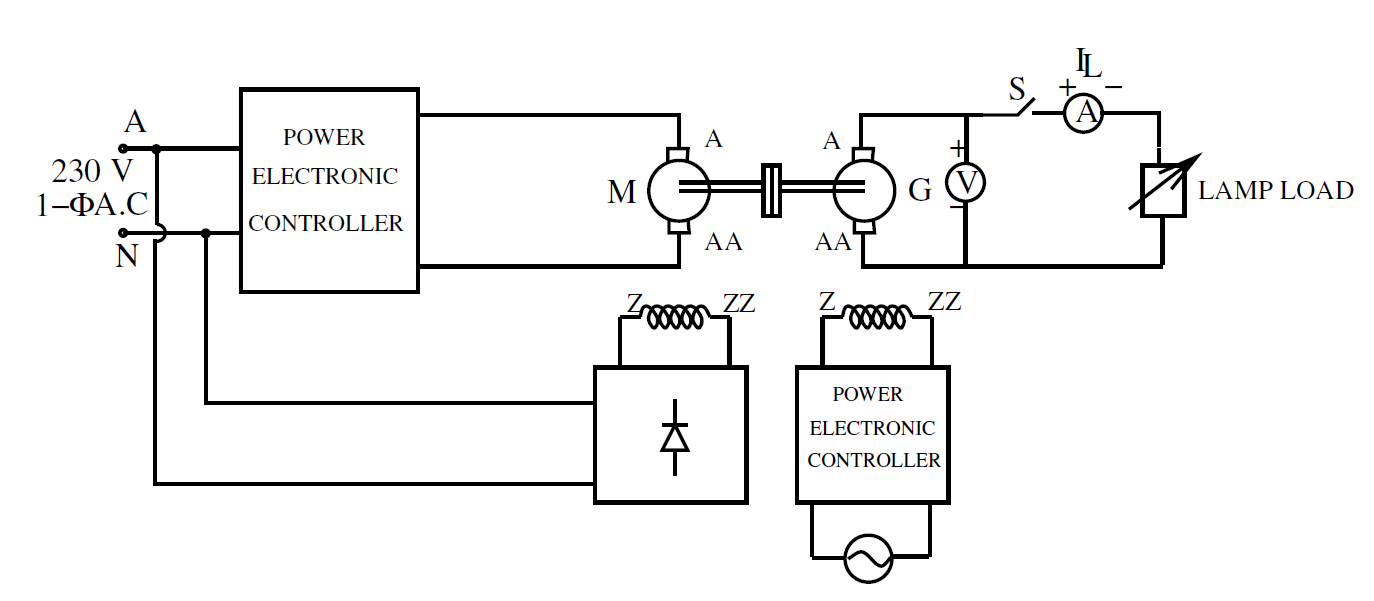
\includegraphics[width = 0.8\linewidth]{LAB-3/sep_ex_gen_circuit.PNG}
                    \caption{Circuit diagram for separately Excited DC Generator(for O.C.C. \& Load test)}
                    \label{fig:my_label}
                 \end{figure}
                 \begin{figure}[H]
                    \centering
                    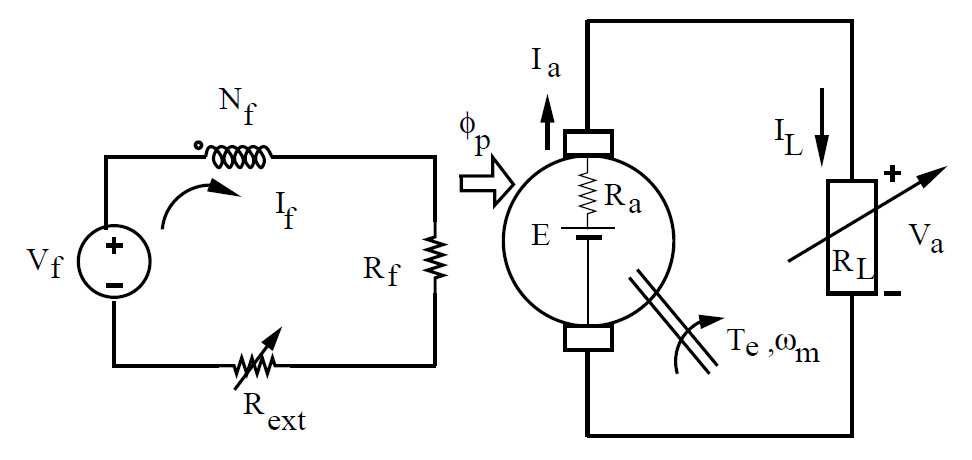
\includegraphics[width = 0.8\linewidth]{LAB-3/sep_equv_cir.PNG}
                    \caption{An Equivalent circuit of a separately excited dc generator}
                    \label{fig:my_label}
                \end{figure}
                \begin{figure}[H]
                    \centering
                    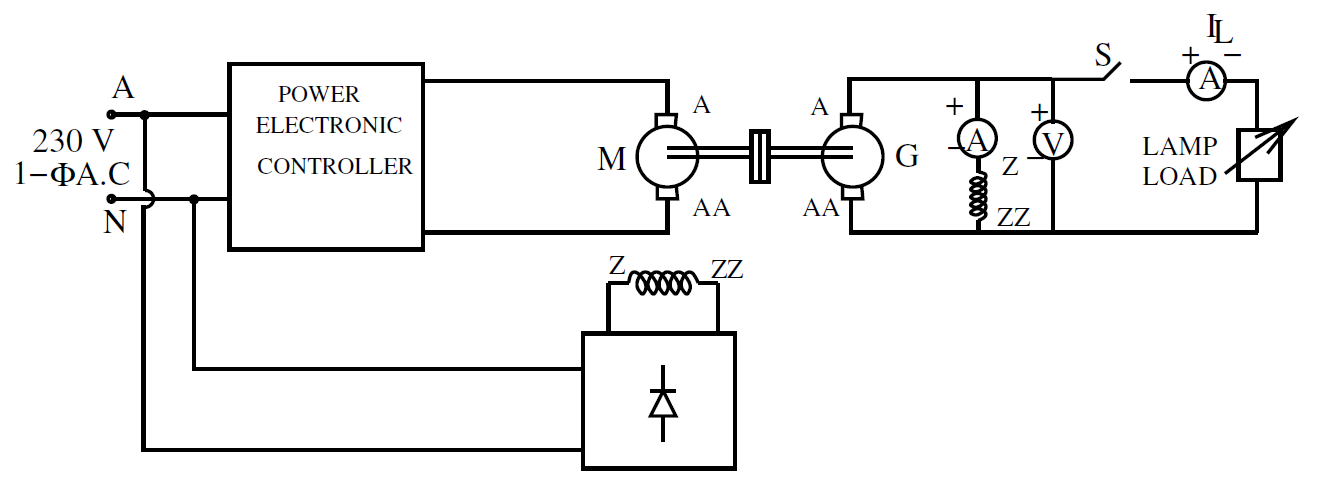
\includegraphics[width = 0.9\linewidth]{LAB-3/shunt_gen_circuit.PNG}
                    \caption{Circuit diagram for separately Excited DC Generator(for O.C.C. \& Load test)}
                    \label{fig:my_label}
                \end{figure}
                \begin{figure}[H]
                    \centering
                    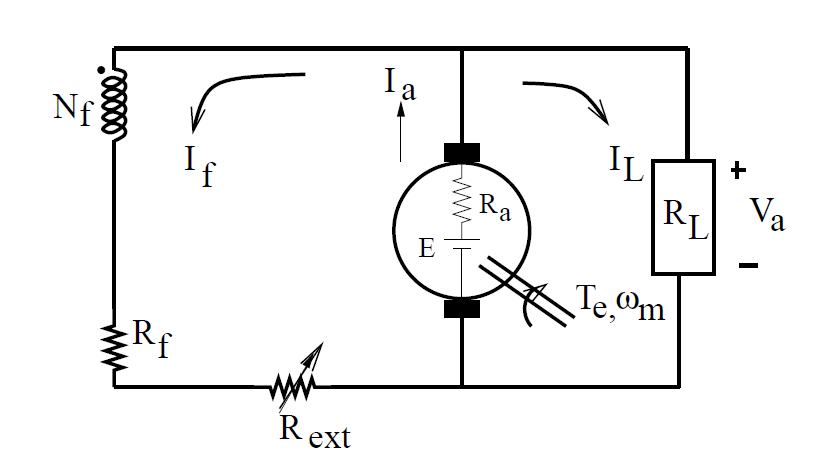
\includegraphics[width = 0.8\linewidth]{LAB-3/shunt_equi_cir.PNG}
                    \caption{An Equivalent circuit of a Self Excited DC generator}
                    \label{fig:my_label}
                \end{figure}
            
    \newpage
    
    \section{Observations}
    \subsection{Seperately excited DC generator}
    \subsubsection{Open circuit characteristics}
    The speed of the dc machine is kept at rated speed of 1500rpm.\\
    The residual magnetism voltage is 10V.
    \begin{table}[ht]
        \centering
        \begin{tabular}{|c|c|c|}
            \hline
            \hline
            Armature Voltage(V) & Field Voltage($V_f$) & Field Current($I_f$) \\
            \hline
            \hline
            10 & 0 & 0 \\
            32	&	22	&	0.05	\\
            60	&	43	&	0.1	\\
            87	&	64	&	0.15	\\
            108	&	83	&	0.2	\\
            128	&	107	&	0.25	\\
            139	&	127	&	0.3	\\
            148	&	151	&	0.35	\\
            155	&	171	&	0.4	\\
            161	&	191	&	0.45	\\
            \hline
        \end{tabular}
        \caption{No-load readings of the dc machine}
        \label{tab:my_label}
    \end{table}
    \vspace{-0.8cm}
    \begin{figure}[ht]
        \centering
        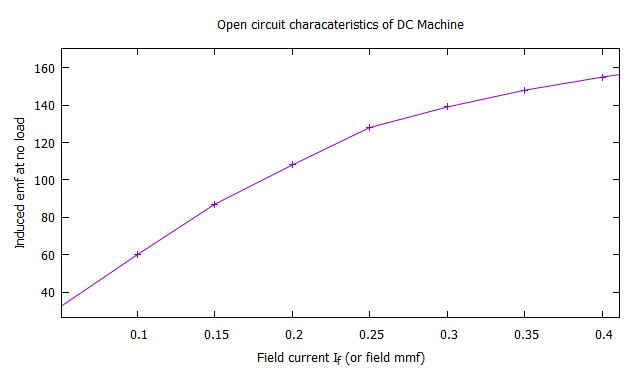
\includegraphics[scale=0.66]{occ.png}
        \caption{No-load characteristics of dc machine}
        \label{fig:my_label}
    \end{figure}
    \newpage
    \subsubsection{External characteristics}
    The speed of the dc machine is kept at rated speed of 1500rpm.\\
    Field voltage is maintained at rated value (196V).
    \begin{table}[ht]
        \centering
        \begin{tabular}{|c|c|c|}
          \hline
            \hline
            No.of Switches & Armature Voltage(V) & Armature Current($I_a$) \\
            \hline
            \hline
            2 &	158	& 0.5\\
            4 &	157	& 1.1\\
            6 &	156	& 1.5\\
            8 &	153 &	2.2\\
            10 &	151 & 2.8\\
            12 &	149 & 3.3\\
            \hline
        \end{tabular}
        \caption{Readings of the dc machine with varying external load}
        \label{tab:my_label}
    \end{table}
    %\vspace{1cm}
    \begin{figure}[ht]
        \centering
        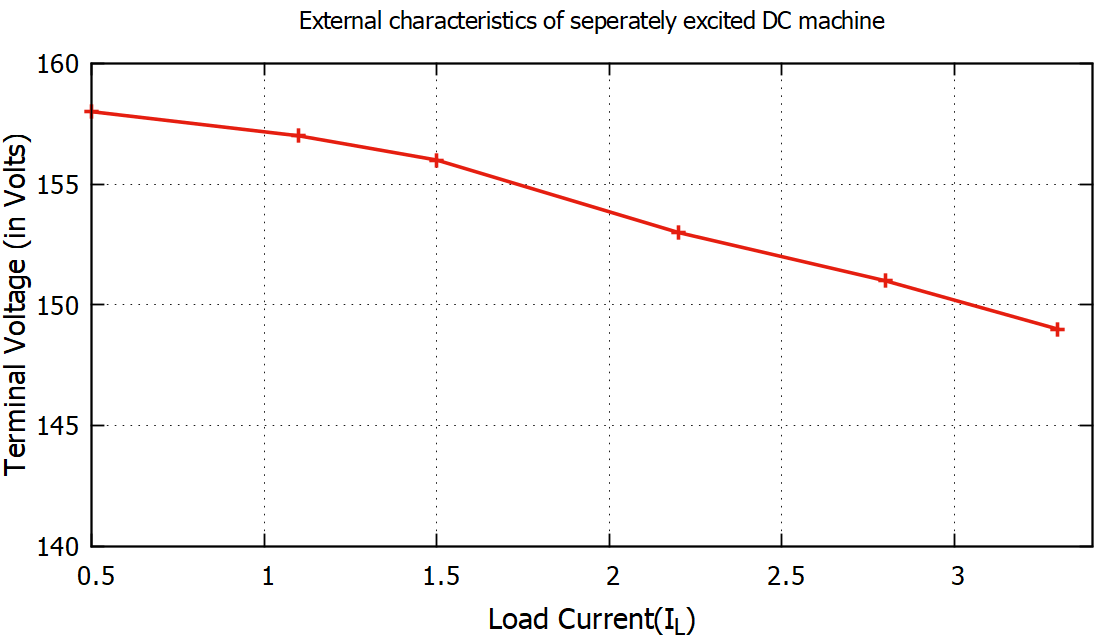
\includegraphics[scale=0.45]{esp.png}
        \caption{External characteristics of separately excited dc generator}
        \label{fig:my_label}
    \end{figure}
    
    %\vspace{1cm}
    \newpage
    \subsection{Self excited generator}
    \subsubsection{External Characteristics}
    The speed of the dc machine is kept at rated speed of 1500rpm.
    \begin{table}[H]
        \centering
        \begin{tabular}{||c||c|c|c|c|c|c||}
          \hline
          \hline
            No.of Load Switches & 2  & 4 & 6 & 8 & 10 & 12 \\
            \hline
            Armature Voltage(V) &	139	& 136 & 134 & 131 & 129 & 126\\
            \hline
            Armature Current($I_a$) & 0.5	& 1.0 & 1.4 & 2 & 2.6 & 3.1\\
            \hline
            Field Current($I_f$) & 0.32 & 0.30 & 0.3 & 0.3 & 0.29 & 0.29\\
            \hline
            Load Current ($I_L=I_a-I_f$)& 0.18 & 0.7 & 1.1 & 1.7 & 2.31 & 2.81 \\
            \hline
            \hline
        \end{tabular}
        \caption{Readings of the self excited generator with varying load}
        \label{tab:my_label}
    \end{table}
    %\clearpage
    \begin{figure}[ht]
        \centering
        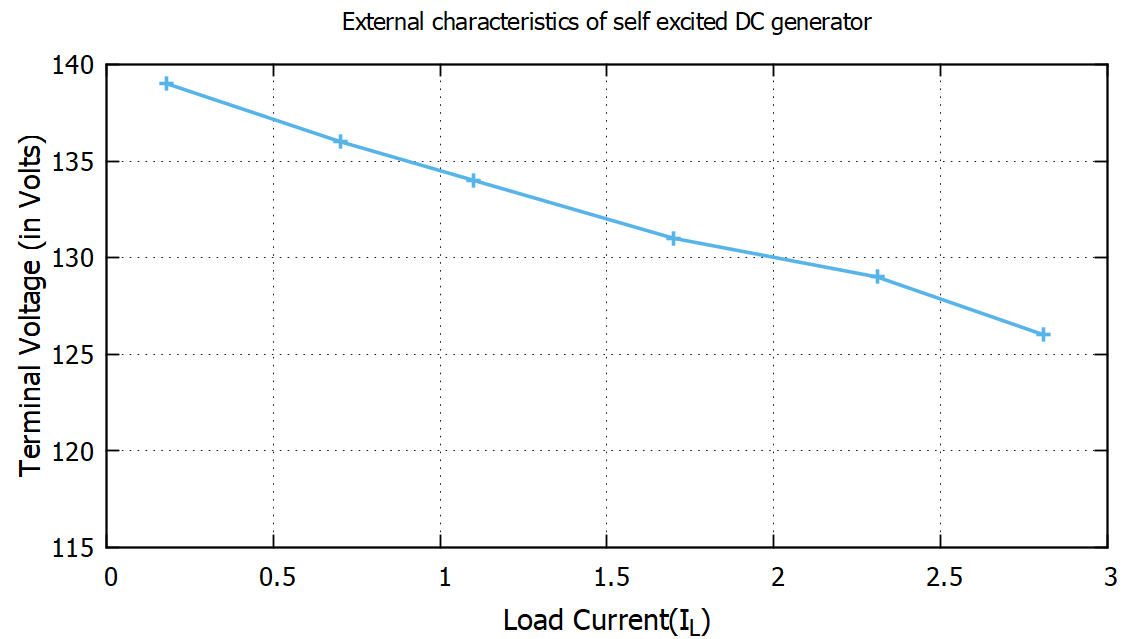
\includegraphics[scale=0.5]{ese.png}
        \caption{External characteristics of self excited DC generator}
        \label{fig:my_label}
    \end{figure}
    \section{Conclusion}
    Hence, from the open circuit characteristics of the dc generator, we observe that the curve is similar to B-H curve (since $E=K_1\phi_f$ and $\phi\alpha I_f$).The constant $K_1$ is dependent on both linear(air) and non-linear(armature, stator) magnetic materials. It is getting saturated as we increase field($\alpha I_f$).
    
    In the external circuit characteristics we observe that the induced voltage(E) vs curve is bent, instead being horizontal. This is because the terminal voltage decreases as current increases, due to armature and load resistance and also due to Armature reaction.
    
    But we observe, this curvature is more seen in self excited, because apart from armature reaction and resistance, the field voltage also gets reduced, since it is in parallel to the induced voltage.
    \section{Post-lab Questions}
     1. Of the two machines which one did you choose to operate as motor? Justify your answer.\vspace{0.1cm}\\
    \textbf{Ans:} The name plate readings of the two machines were as follows:
    \begin{itemize}
    \item 1.5 kW DC machine: $R_a = 2:04\Omega, R_F = 415\Omega,$ Friction wind-age loss at 1500 rpm = 53W. 
    \item 1.1 kW DC machine: $R_a = 2:1\Omega, R_F = 415\Omega,$ Friction wind-age loss at 1500 rpm = 53W.
    %are these readings enough to justify or they are redundant to specify the input and output machine 
    \end{itemize}
    
    The machine with high rated output power should be used in input. The machine features are all almost the same with just difference in the rated output power, and in this experiment we are using a motor(input) to drive a generator(output). Hence 1.5 kW DC machine should be used as a motor and the other DC machine as generator.
    \vspace{0.1cm}\\
    2. Assume that a given machine has the following name plate ratings: 220 V, 1.5 kW, 1500 rpm dc generator What do these numbers imply?\vspace{0.1cm}\\
    \textbf{Ans:}\\
        $220\ V$ - \textbf{Rated voltage}: Maximum voltage that can be applied(motor)/Observed(generator) to the DC machine.(If above, the machine might damage either in short term or in long term).\\%not sure what it means for a generator
        $1.5\ kW$ - \textbf{Rated output power}: Power generated at the final output(after removing all the losses) when rated voltage is applied(motor)/Observed(generator) at rated torque.\\%not sure what it means for a generator
        $1500\ rpm$ - \textbf{Base speed}: The speed at which the DC motor rotates at rated voltage and rated current, the speed at which the DC generator should be operated for realising Rated voltage.%why is the DC generator should be operated at a specific speed, if the motor is usually operated at different speeds.   
    \vspace{0.1cm}\\
    3. There are motors without any rotor winding ( e.g. stepper motor). Explain how the torque is produced in these machines ( Hint: Go through very carefully the theory given in the first page).\vspace{0.1cm}\\
    \textbf{Ans:} The torque generation is based on the principle of alignment of two magnetic fields, a magnet placed in a magnetic field experiences torque unless and until its magnetic field is aligned with the external magnetic field.
    There are machines whose rotors do not have any winding but instead the rotor is itself an electromagnet which has a fixed magnetic field direction, to rotate the rotor a variable directional magnetic field is applied through the stator and the rotor rotates to align its magnetic field to the external magnetic field(stator).
    \vspace{0.1cm}\\
    4. How is the voltage induced in the armature (coil is rotating in a magnetic field) which is ac, converted to dc?\vspace{0.1cm}\\
    \textbf{Ans:} Let's consider one coil of the rotor, if the coil ends are directly taken out and connected to the terminals of a voltmeter, the voltage across those terminals would be AC. So the ends are interchanged(to the terminals of output voltage) as soon as the coils change their current direction using commutator. This rectifies only partially as the output voltage is converted from positive and negative cycles to only positive cycles, the constant voltage is obtained by using many rotor coils, voltage generated by each of these coils would be shifted in time with respect to each other which adds up to a constant voltage at the output.
    \vspace{0.1cm}\\
    5. What is the effect of armature reaction?\vspace{0.1cm}\\
    \textbf{Ans:} As a result of armature reaction,
    \begin{itemize}
        \item The resultant flux gets distorted. It is not aligned along the symmetric axis of the two poles.
        \item The overall flux density gets slightly reduced. On one half of a pole it increases and on the other half of it, it decreases.
        \item It induces flux in the neutral zone, and this flux generates the voltage that causes the commutation problem.
    \end{itemize}
    \vspace{0.1cm}\\
    6. `Saturation of the magnetic material is a blessing in the case of self excited generator' Is this statement true? Justify your answer. (Hint: comment on the following:\\
     Voltage build up is cumulative in nature if the generator is operated in the linear region of the magnetization curve.)\vspace{0.1cm}\\
    \textbf{Ans:} In self excited generators, voltage build up is cumulative in nature if the generator is operated in the linear region of the magnetizing core as the increase in the emf of the generator increases the field current which corresponds to increase in the flux which thereby increases the emf of the generator, this continues until the core is saturated and any increment in emf doesn't increase the flux in the core.
    
    Now if there is no saturation of the magnetic material, the output voltage keeps on increasing(in the case of air core types) which eventually exceeds the rated voltage which implies that the machine might get damaged as a cause of high voltage.
    \vspace{0.1cm}\\
    7. In separately excited dc machine, the field winding carries a constant current. Hence, it dissipates power. Suggest a method to eliminate this power loss.\vspace{0.1cm}\\
    \textbf{Ans:} To reduce power loss, field current has to be reduced. But we need high field flux, we can increase the number of turnings of the coil to get the same flux with small current thereby reducing the power loss  
    \vspace{0.1cm}\\
    8. What may happen if load terminals are short circuited in (a) separately excited generator (b) self excited generator\vspace{0.1cm}\\
    \textbf{Ans:} We might expect that shorting always leads to damage of the circuit, but this is not exactly shorting as there is always armature resistance.
    
    (a) In separately excited generator, shorting terminals leads to large current flow in the circuit (when field flux is large) which results to burning of the wire and the wire opens up, the circuit becomes an open circuit, in this process the internals of the generator might get damaged.% not sure 
    
    (b) In self excited generator, shorting terminals ensures no current flow in the field coil. So voltage build up doesn't occur and hence the initial voltage(due to residual flux) remains the same. As there is armature resistance current flows(not very large as the residual emf is not very large) through the shorted circuit but not through the field coils.
    \vspace{0.1cm}\\
    9. You have been given the plot of Efficiency Vs input power of the prime mover. Explain how will you obtain the plot of efficiency Vs output power of the generator. How will you obtain this plot in-case the plot of Efficiency Vs input power of the prime mover is not available?\vspace{0.1cm}\\
    \textbf{Ans:} If the efficiency vs input power plot is given to us, we can obtain input power with the it. Then dividing the output power with the obtained input voltage would just give us the overall efficiency.
    
    But in case, the efficiency plot is not given to us, then we can manually get output and input power values by using multimeters across load and the armature.
    
    \vspace{0.1cm}\\
    
    %\begin{thebibliography}{}
    %\bibitem{LAB Manual}
     %   DC Generator characteristics\\
      %  \\
    %https://moodle.iitb.ac.in/pluginfile.php/295441/mod\_forum/attachment/208441/DCGeneratorCharacterstics.pdf
    
    %\end{thebibliography}
    
\end{document}